\chapter{Model matematyczny}
\label{cha:model_matematyczny}

\section{Model silnika elektrycznego prądu stałego}
Silnik elektryczny odpowiedzialny za poruszanie ramieniem został zamodelowany jako obiekt inercyjny pierwszego rzędu. Równania \ref{ele1} i \ref{ele2} opisują zależność generowanego momentu obrotowego od prądu.
\begin{equation}\label{ele1}
M(t) = k_e \cdot i(t)
\end{equation}
\begin{equation}\label{ele2}
U(t) = i(t) \cdot R + L \cdot \frac{di(t)}{dt}
\end{equation}
\noindent gdzie:\\
$M(t)$ - moment generowany przez silnik,\\
$i(t)$ - prąd elektryczny,\\
$k_e$ - stała elektryczna silnika,\\
$L$ - indukcyjność silnika,\\
\(R\) - opór elektryczny silnika.

\section{Model matematyczny obiektu}
Równania mechaniczne opisujące dynamikę całego układu mają postać:\\
\begin{equation}\label{r1}
\frac{d^2 \alpha(t)}{dt^2} \cdot J = k_e \cdot i(t) 
\end{equation}
\begin{equation}\label{r2}
U(t) = i(t) \cdot R + \frac{d i(t)}{dt} \cdot L
\end{equation}
gdzie:\\
$\alpha$ - kąt wychylenia,\\
$J$ - moment bezwładności ramienia,\\
$U(t)$ - napięcie podawane na silnik.\\

W przyjętym modelu obiektu założono, że wielkością sterującą jest napięcie podawane na silnik, a wyjściową kąt wychylenia ramienia.\\
Na podstawie równań \ref{r1} i \ref{r2} zapisano model matematyczny w postaci równań stanu, przyjmując następujące zmienne stanu:\\
$x_1$ - prąd silnika\\
$x_2$ -  położenie kątowe ramienia\\
$x_3$ - prędkość kątowa ramienia\\
\begin{equation}\label{key}
\dot {x_1} = -x_1  \cdot \frac{R}{L} + \frac{U}{L}
\end{equation}
\begin{equation}\label{key}
\dot {x_2} = x_3
\end{equation}
\begin{equation}\label{key}
\dot {x_3} = \frac{k_e}{J} \cdot x_1
\end{equation}

Schemat blokowy realizujący powyższe równania stowrzono z wykorzystaniem programu \textit{Simulink} oraz przedstawiono na rysunku \ref{fig:model}. 

\begin{figure}[h]
	\centering
	\includegraphics[width=4in]{Figures/model.png}
	\caption{Schemat blokowy programu \textit{Simulink}.}
	\label{fig:model}
\end{figure}

Na rysunkach \ref{fig:step1} - \ref{fig:step3} przedstawiono odpowiedzi poszczególnych zmiennych stanu na skok napięcia.

\begin{figure}[h]
	\centering
	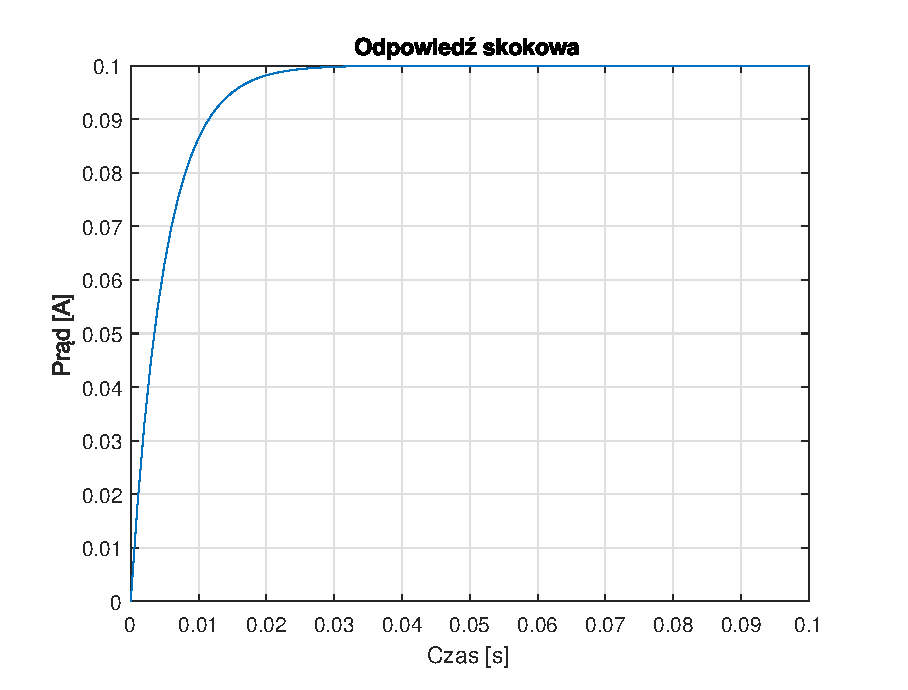
\includegraphics[width=4in]{Figures/step_curr.eps}
	\caption{Odpowiedź prądu na skok napięcia.}
	\label{fig:step1}
\end{figure}

\begin{figure}[h]
	\centering
	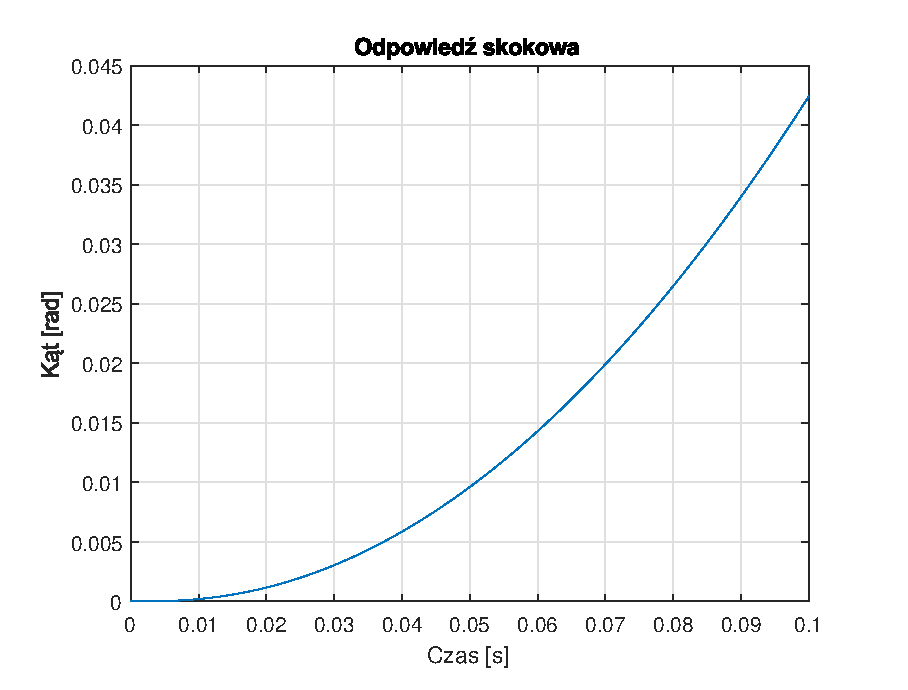
\includegraphics[width=4in]{Figures/step_ang.eps}
	\caption{Odpowiedź kąta na skok napięcia.}
	\label{fig:step2}
\end{figure}

\begin{figure}[h]
	\centering
	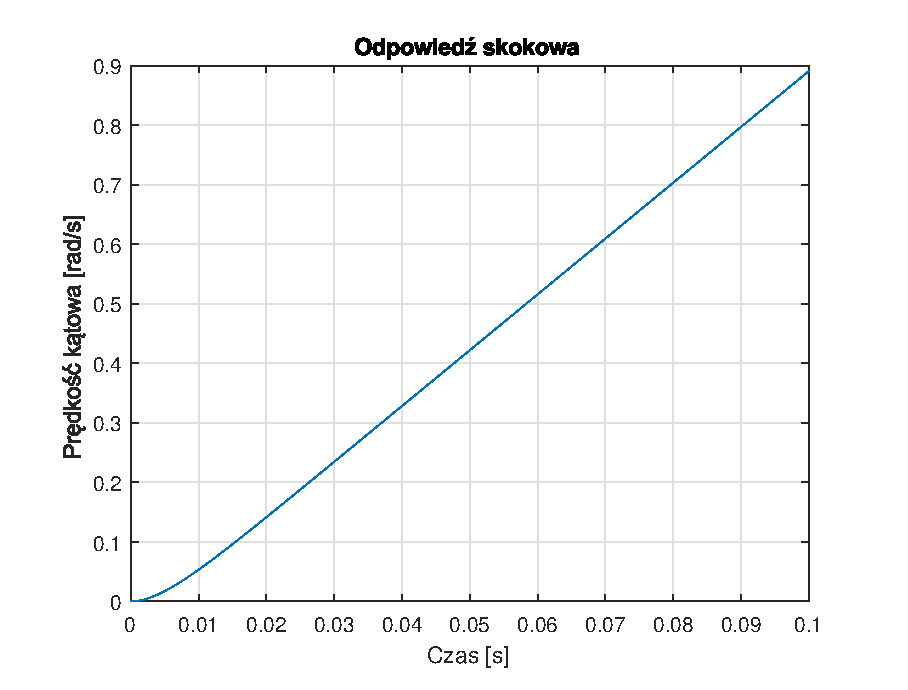
\includegraphics[width=4in]{Figures/step_vel.eps}
	\caption{Odpowiedź prędkości kątowej na skok napięcia.}
	\label{fig:step3}
\end{figure}